\documentclass[noabstract,doubleheaders,onlytitle,titlepage,oneside,openright,11pt]{epflthesis}
% \documentclass[doubleheaders,los,lof,lot,titlepage,oneside,openright,11pt]{epflthesis}
\includeonly{chapters/basics}

\usepackage{array}
\usepackage[margin=3cm]{geometry}
\usepackage[linesnumbered,ruled]{algorithm2e}
\usepackage{float}
\usepackage{xcolor}
\usepackage{graphicx}
\usepackage{amsmath}
\usepackage{siunitx}
\usepackage{placeins}
\usepackage{xfrac}
\usepackage{caption}
\usepackage{subcaption}
\usepackage{booktabs}
\usepackage{tabularx}
\usepackage{multirow}
\usepackage[utf8]{inputenc}
\usepackage[T1]{fontenc}
\usepackage{lmodern}
\usepackage{hyperref}
\usepackage{etoolbox}
\usepackage{bm}
\usepackage{amssymb}
\usepackage[xindy,nogroupskip,section,indexonlyfirst]{glossaries}
\usepackage{glossary-katie}
\usepackage[toc,page]{appendix}

\usepackage{tikz}
\usepackage{pgfplots}
\usetikzlibrary{calc}

\usepackage{rotating}
\usepackage{relsize}
\usepackage{xstring}
\usepackage{kbordermatrix}
\usepackage{ragged2e}

\renewcommand{\u}[2]{\ensuremath{\SI{#1}{#2}}}
\newcommand{\mlab}{\texttt{MATLAB}}
\newcommand{\emlab}{\texttt{Embedded MATLAB}}
\newcommand{\slink}{\texttt{Simulink}}
\newcommand{\cpp}{C\nolinebreak[4]\hspace{-.05em}\raisebox{.4ex}{\relsize{-3}{\textbf{++}}}}
\newcommand{\eigen}{\texttt{Eigen }}
\newcommand{\ros}{\texttt{ROS }}
\newcommand{\rviz}{\texttt{rviz }}
\newcommand{\rovio}{\texttt{rovio }}
\newcommand{\opencv}{\texttt{opencv }}
\newcommand{\cholmod}{\texttt{CHOLMOD}}
\newcommand{\argmin}[1]{\underset{#1}{\operatorname{arg}\,\operatorname{min}}\;}
% string commands
\newcommand{\ReplaceStr}[2]{%
  \IfSubStr{#1}{XX}{%
    \StrSubstitute{#1}{XX}{#2}
  }{#1}
}

% glossary shortcuts
\newcommand{\g}[1]{\gls*{#1}}
\newcommand{\gi}[1]{\glsuseri*{#1}\glsunset{#1}}
\newcommand{\gii}[1]{\glsuserii*{#1}\glsunset{#1}}
\newcommand{\giii}[1]{\glsuseriii*{#1}\glsunset{#1}}
\newcommand{\giv}[1]{\glsuseriv*{#1}\glsunset{#1}}
\newcommand{\gv}[1]{\glsuserv*{#1}\glsunset{#1}}

\newcommand{\ga}[1]{\glsuseri*{#1}\glsunset{#1}}
\newcommand{\gb}[1]{\glsuserii*{#1}\glsunset{#1}}
\newcommand{\gc}[1]{\glsuseriii*{#1}\glsunset{#1}}

\newcommand{\gk}[1]{\gls*{#1}}
\newcommand{\gpo}[1]{\glsuseri*{#1}\glsunset{#1}}
\newcommand{\gmo}[1]{\glsuserii*{#1}\glsunset{#1}}
\newcommand{\gpi}[1]{\glsuseriii*{#1}\glsunset{#1}}
\newcommand{\gpio}[1]{\glsuseriv*{#1}\glsunset{#1}}

\newcommand{\gentry}[1]{\glsentryname{#1}}
\newcommand{\gentryi}[1]{\glsentryuseri{#1}}
\newcommand{\gentryii}[1]{\glsentryuserii{#1}}
\newcommand{\gentryiii}[1]{\glsentryuseriii{#1}}
\newcommand{\gentryiv}[1]{\glsentryuseriv{#1}}

\newcommand{\gentrymo}[1]{\glsentryuserii{#1}}

\newcommand{\addsym}[2]{#1\addsymbol{#1}{#2}}
\newcommand{\addlat}[4][]{%
  \ifstrempty{#1}{\def\mysort{#2}}{\def\mysort{#1}}
  \glssetexpandfield{sortvalue}
  \newglossaryentry{#2}{name={#3},description={#4},type={latin},sort=\mysort}
}
\newcommand{\addgrk}[4][]{%
  \ifstrempty{#1}{\def\mysort{#2}}{\def\mysort{#1}}
  \glssetexpandfield{sortvalue}
  \newglossaryentry{#2}{name={#3},description={#4},type={greek},sort={\mysort}}
}

\newcommand{\addlatdelta}[4][]{
  \ifstrempty{#1}{\def\mysort{#2}}{\def\mysort{#1}}
  \glssetexpandfield{sortvalue}
  \newglossaryentry{#2}{name={#3},user1={\gentryi{Delta}#3},description={#4},type={latin},sort={\mysort}}
}

\newcommand{\addlatnumbered}[4][]{%
  \addglsnumbered{#1}{#2}{#3}{#4}{latin}%
}

\newcommand{\addgrknumbered}[4]{%
  \addglsnumbered{#1}{#2}{#3}{#4}{greek}%
}

\newcommand{\addglsnumbered}[5]{%
  \saveexpandmode\normalexpandarg
  \saveexploremode\exploregroups
  \StrSubstitute{#3}{XX}{}[\myname]%
  \StrSubstitute{#3}{XX}{,1}[\myuserone]%
  \StrSubstitute{#3}{XX}{,2}[\myusertwo]%
  \restoreexpandmode
  \restoreexploremode
  \glssetexpandfield{sortvalue}
  \glssetexpandfield{name}
%
  \ifstrempty{#1}{\def\mysort{#2}}{\def\mysort{#1}}
  \newglossaryentry{#2}%
  {%
    name={\myname},%
    user1={\myuserone},%
    user2={\myusertwo},%
    description={#4},%
    sort={\mysort},%
    type={#5}%
  }%
}

\newcommand{\addlatelement}[4][]{%
  \addglselement{#1}{#2}{#3}{#4}{latin}%
}

\newcommand{\addglselement}[5]{%
  \ifstrempty{#1}{\def\mysort{#2}}{\def\mysort{#1}}%
  \newglossaryentry{#2}%
  {%
    name={\ensuremath{\vc{#3}}},%
    user1={\ensuremath{#3_i}},%
    user2={\ensuremath{#3_{i,j}}},%
    user3={\ensuremath{\vc{\hat{#3}}}},%
    description={test}%
    sort={\mysort},%
    type={#5}%
  }%
}


\newcommand{\addlatfork}[4][]{%
  \addglsfork{#1}{#2}{#3}{#4}{latin}%
}

\newcommand{\addgrkfork}[4][]{%
  \ifstrempty{#1}{\def\mysort{#2}}{\def\mysort{#1}}
  \addglsfork{\mysort}{#2}{#3}{#4}{greek}%
}

\newcommand{\addglsfork}[5]{%
  \saveexpandmode\normalexpandarg
  \saveexploremode\exploregroups
  \StrSubstitute{#3}{XX}{k}[\myname]%
  \StrSubstitute{#3}{XX}{k+1}[\myuserone]%
  \StrSubstitute{#3}{XX}{k-1}[\myusertwo]%
  \StrSubstitute{#3}{XX}{k+i}[\myuserthree]%
  \StrSubstitute{#3}{XX}{k+i+1}[\myuserfour]%
  \restoreexpandmode
  \restoreexploremode
  \glssetexpandfield{sortvalue}
  \glssetexpandfield{name}
%
  \ifstrempty{#1}{\def\mysort{#2}}{\def\mysort{#1}}
  \newglossaryentry{#2}%
  {%
    name={\myname},%
    user1={\myuserone},%
    user2={\myusertwo},%
    user3={\myuserthree},%
    user4={\myuserfour},%
    description={#4},%
    sort={\mysort},%
    type={#5}%
  }%
}

% underbrace with normal text
\newcommand{\ubrace}[2]{\underbrace{#1}_{\textstyle #2}}
\newcommand{\obrace}[2]{\overbrace{#1}^{\textstyle #2}}


\newcommand{\dt}[1]{\ensuremath{\frac{d#1}{dt}}}
\newcommand{\ut}[1]{\ensuremath{_\text{#1}}}

% define what to do with vectors
\newcommand{\vc}[1]{\ensuremath{\bm{#1}}}

% transpose
\newcommand{\tps}[1]{\ensuremath{#1^\intercal}}

% add argmin operator in math mode
%\DeclareMathOperator*{\argmin}{arg\,min}

% redefine ams macro to allow optional argument for controlling matrix line spacing
\makeatletter
\renewcommand*\env@matrix[1][\arraystretch]{%
  \edef\arraystretch{#1}%
  \hskip -\arraycolsep
  \let\@ifnextchar\new@ifnextchar
  \array{*\c@MaxMatrixCols c}
}
\makeatother

% command to add extra space between rows of an amsmath matrix
\newcommand{\matskip}[1]{\\\noalign{\vspace{#1}}}

% remove header info from glossaries
\renewcommand{\glsglossarymark}[1]{}

\newcommand{\imp}[1]{\centering \textbf{\textcolor{ETHlightishblue}{#1}}}

\definecolor{myblue}{RGB}{70, 170, 210}
\definecolor{mygreen}{RGB}{80, 170, 80}

\setglossarystyle{long}

\newglossary*{latin}{Symbols}
% Optimization
\addlatelement[a]{a}{a}{Spline coefficients}
\addlatelement[xi]{xi}{\ensuremath{\xi}}{Camera pose}
\addlatcameras[r]{r}{r}{Residual vector}
\addlatcameras[u]{u}{XX u}{Pixel vector}
\addlatcameras[uu]{uu}{XX \tilde{u}}{Undistorted pixel vector}
\addlatcameras[w]{w}{XX \tilde{w}}{Rectified pixel vector}
\addlatcameras[I]{I}{I}{Image intensity function}
\addlatiterations[Jrs]{Jrs}{\ensuremath{\vc J_rXX(\vc a)}}{Photometric error Jacobian with respect to spline coefficients}
\addlatiterations[Jrp]{Jrp}{\ensuremath{\vc J_rXX(\vc \xi)}}{Photometric error Jacobian with respect to camera position}
\addlat[Jf]{Jf}{\ensuremath{\vc J_f(\vc a)}}{Cost function Jacobian}
\addlat[B]{B}{\ensuremath{\vc B}}{Bending energy matrix}
\addlat[G]{G}{\ensuremath{\vc G}}{Gradient energy matrix}

\addlat[pk]{pk}{\ensuremath{\vc p^k_{GN}}}{Gauss-Newton optimization direction}
\addlat[N]{N}{N}{Number of map points}
\addlat[M]{M}{M}{Number of spline coefficients}
\addlat[K]{K}{K}{Number of camera positions}
\addlat[s]{s}{s}{Support of spline functions}
\addlatelement[x]{x}{\ensuremath{x}}{3D map coordinates}

% Camera parameters
\addlat[Kk]{Kk}{\ensuremath{\vc K_k }}{Camera matrix (intrinsic parameters)}
\addlat[Kprime]{Kprime}{\ensuremath{\vc K_k'}}{Rectified camera matrix (intrinsic parameters)}
\addlat[Dk]{Dk}{\ensuremath{D_k}}{Camera distortion function (intrinsic parameters)}
\addlat[R]{R}{\ensuremath{\vc{R}_k}}{Passive stereo to camera rotation matrix}
\addlat[Tk]{Tk}{\ensuremath{\vc T_k}}{Object to camera space transformation}
\addlat[Proj]{Proj}{\text{Proj}}{Object to image space transformation}
\addlat[pi]{pi}{\ensuremath{\vc \pi}}{Pinhole camera projection}
\addlat[b]{b}{\ensuremath{b}}{Camera baseline}
\addlat[fx]{fx}{\ensuremath{f_x}}{Camea focal width}
\addlat[fy]{fy}{\ensuremath{f_y}}{Camea focal height}

\addlat[rab]{arab}{\ensuremath{{_{A}\vc{r}_{AB}}}}{Vector from Point $A$ to $B$
  expressed in coordinates $\mathcal{A}$}
\addlat[cba]{cba}{\ensuremath{\vc{C}_{BA}}}{Passive rotation matrix from
  coordinate frame $\mathcal{B}$ to $\mathcal{A}$.} 
\addlat[phiba]{phiba}{\ensuremath{\vc{\Phi}_{BA}}}{Passive rotation vector from
coordinate frame $\mathcal{B}$ to $\mathcal{A}$.}
\addlat[C]{C}{\ensuremath{\vc{C}}}{Rotation transformation from $SO(3)$ to
  $\mathbb{R}^{3\times3}$}

% Indices
\addlat[Mf]{Mf}{\ensuremath{\mathcal{M}}}{Map coordinate frame}
\addlat[Cf]{Cf}{\ensuremath{\mathcal{C}}}{Camera coordinate frame}
\addlat[Sf]{Sf}{\ensuremath{\mathcal{S}}}{Stereo coordinate frame}

\makeglossaries

\title{Visual Terrain Estimation For Legged Robots}
\author{Frederike Dümbgen}
\advisor{Alireza Karimi (EPFL)\\
Michael Blösch (ETHZ) \\
Philipp Krüsi (ETHZ) \\
Dominik Schindler (ETHZ) }
\submitdate{29 July 2016}
\school{Ecole polytechnique fédérale de Lausanne}
\dept{Mechanical Engineering}
% \logo{figures/ABB_logo_small.png}
\city{Zurich}

\printlos{%
  \printglossary[type=latin]
  % \printglossary[type=greek]
}


\begin{document}

% \maketitle
% \tableofcontents
% \chapter*{Symbols}
% \printglossaries

\section{Introduction}

\subsection{Motivation}
\frame{
  \frametitle{Dense SLAM with B-Splines}

  Picture of Sparse SLAM 
  Picture of Dense SLAM
}

\subsection{Project Goals}
\frame{
  \frametitle{Project Goal and Methodology}

  Create framework for surface reconstruction and localization using moving
  stereo camera based on moving monocular camera case. 

  \begin{columns}
    \column{0.35\textwidth}

    Added functionalities
    \begin{itemize}
      \item Create spline surface reprensentation from static stereo camera.  
      \item Localize new stereo camera position using obtained map.
    \end{itemize}

      \column{0.65\textwidth}
    Methodology
    \begin{itemize}
    \item Simulation environment \ros with \rviz for pointcloud and
      \opencv for image handling.
      \item Implementation of optimization algorithm using \eigen 's
      sparse matrix solvers.
      \item Localization method using photometric errors only and generic
        rotation representation
    \end{itemize}
  \end{columns}
}


\chapter{Notation and Basics}
\section{Geometry}
\subsection{Vectors and Coordinate Frames}

The vector and coordinate frame notations used throughout this report follow the
conventions introduced in \cite{coordinates}.
If \g{Mf} is the coordinate frame associated with the map, and $A$, $B$ are two 
3D points, then \g{arab} contains the coefficients of the vector pointing from $A$ to $B$ expressed in the map coordinate system.
In the same manner, the rotation matrix \g{cba} is the (passive) matrix linking
the coordinates in a frame $\mathcal{A}$ to the coorindates in $\mathcal{B}$ like

\begin{equation}
  \brab = \g{cba} \left( \g{arab} \right) \text{ .}
\end{equation}

\subsection{Rotation Representations}

For convenient handling of rotations, i.e. their derivatives and updates, the
rotation vectors \Phic, \Phis $\in\mathbb{R}^3$ are introduced as recommended in 
\cite{Primer} to represent the relative orientations of the stereo and camera
frames with respect to the map frame, respectively. The corresponding updates in
rotation are denoted by \phic and \phis.

The new rotation $\Phic^{k+1}$, resulting from a relatively small change in
rotation \phic, can be conveniently expressed using the $\boxplus$-operator as

\begin{align}
  \Phic^{k+1} &= \Phic^k \boxplus \phic \\
  &= \exp(\phic) \circ \Phic^k \\
  &= \vc C(\phic) \vc C(\Phic^k)  
\end{align}

The mapping $\g{C} : SO(3) \implies \mathbb{R}^{3\times3}$ applied to the
orientation vector \Phic corresponds to the rotation matrix \rotcm since it is
defined as
\begin{align}
  \Phic(\vc{r}) &:= \g{C}(\Phic)\vc{r} \\
  &= \rotcm(\vc{r})
  \label{eq:basics-rotation} \text{ .}
\end{align}

The transformation defined in \ref{eq:basics-rotation} can be derived with
respect to the orientation vector \Phic and the vector $\vc{r}$, yielding

\begin{align}
  \pderiv{\Phic(\vc {r})}{\vc r} = \g{C}(\Phic) \text{ ,} \quad 
  \pderiv{\Phic(\vc {r})}{\vc \Phi} = -(\Phic(\vc r))^\times
  \text{ ,}
\end{align}

and

\begin{equation}
  \pderiv{(\Phic \circ \Phis)(\vc {r})}{\Phis} = \g{C}(\Phic) \text{ .}
\end{equation}

\section{Camera}
\subsection{Camera Model}

Having introduced the orientation vectors, the camera poses can be described by
\begin{align*}
  \g{xi}_{C_k} &:= \rowvector{\mrmc & \phic}^T \\
  \g{xi}_S &:= \rowvector{\mrms & \phis}^T \text{ .}
\end{align*}

The transformation from object space coordinates \mrmx to pixel coordinates
\giv{u} can be split up in the transformation 
      
\begin{equation*}
  \crcx = \rotcm (\mrmx - \mrmc) \text{, }
\end{equation*}

which is essentially a coordinate transformation from the map frame to the camera
frame using the camera's extrinsic parameters, and 

\begin{equation}
  \giv{u} = \g{Kk} \g{Dk}(\g{pi}(\crcx)) \text{, }
  \label{eq:unrectified}
\end{equation}

which assigns a pixel value to each camera coordinate using the camera model and
its intrinsic parameters.

The model used to approximate the real camera is a pinhole model suspect to
radial - tangential distortion. A pinhole model assigns to each point \crcx
its projection

\begin{equation}
  \g{uu} = \g{pi}(\crcx) = \rowvector{x/z & y/z & 1}^T
\end{equation}

The obtained normalized coordinates \g{uu} are then distorted using the distortion model \g{Dk} defined by
\cite{radtan}, which can be scaled and shifted using the camera matrix \g{Kk} in order to
give pixels the final pixels \rowvector{u, v} lying in \rowvector{0\ldots w,0\ldots h}.

\subsection{Stereo Parameters}

The same considerations as above can be made when unrectified instead of
rectified images are available. The camera calibration in general provides us
with information on the orientations of the cameras with respect to the
rectified image plane \g{R} and their baseline \g{b}. \cite{DocCameraInfo}
\cite[p.  523f]{Siciliano2007}
In the present notation, this means in particular that 

\begin{equation}
  \rotsc = \g{R} \hspace{1em} \text{and} \hspace{1em} \srcc = \g{b} 
  \label{rect/eqn:assumptions}
\end{equation}

are known. The distortion coefficients \g{Dk} are zero and the obtained normalized
points need to be rotated to lie in the same rectified image plane. The camera projection
\ref{eq:unrectified} for the rectified case therefore becomes

\begin{equation*}
  \giv{w} = \g{Kprime}\g{R}(\g{pi}(\crcx)) \text{,}
\end{equation*}

where \g{Kprime} is a modified camera matrix which, depending on the
camera calibration, can be used to scale the image to void non-defined
image borders resulting from image undistortion and rectification. 

For a given set of rectified and unrectified images of a well calibrated camera,
there are strong correspondances between the pixels obtaiend from projections of
3D points to the rectified and the unrectified images respectively. This
connection was exploited to test the correctness of the above transformations 
and the provided camera paramteres, as shown in Appendix \ref{app:parameters}.

\subsection{Interpolation}

The image has to be interpolated around the obtained floating-precision pixel
locations using any common interpolation kernel $h(i, j)$ and summing over 

\begin{align}
  I(x, y) &= \summ{i}{s} \summ{j}{s} I(x_i, y_j) h(i, j) \\
  &= \summ{i}{s} \summ{j}{s} I(x_i, y_j) h(i) h(j)
  \label{eq:basics:interpolation}
\end{align}

The indices $x_i$ and $y_i$ correspond to the location of the image where the
interpolation function $h(i, j)$ takes its maximum value.

The applied scheme in this project was the 
Keys cubic convolution interpolation kernel \cite{Keys1981}, defined by
\begin{equation}
  h(x) = 
  \begin{cases}
     0.5(x - 2)^3 + 2.5(x-2)^2+4(x-2) + 2 & \ 0 \leq x < 1 \\
     -1.5(x-2)^3 - 2.5(x-2)^2 + 1 & \ 1 \leq x < 2 \\
     1.5(x-2)^3 - 2.5(x-2)^2 + 1 & \ 2 \leq x < 3 \\
     -0.5(x -2)^3 + 2.5(x-2)^2 - 4(x-2) + 2.0 & \ 3 \leq x < 4 \\
  \end{cases}
\end{equation}

Other choices of interpolation schemes, such as bilinear or quadratic
interpolation kernels, could have been considered but no further investigation 
was done in this direction since the interpolation scheme did not show any 
significant effect on the results. 

\subsection{Disparity Images} 

In order to quantify the error between the obtained 3D map and the reference
map, disparity images of both maps are created and their difference is evaluated. 
This approach is preferred over other approaches such as the sum over all height
differences, since at sharp edges a little lateral offset can induce very
high differences, but the disparity map's error stays relatively constrained, depending 
on the resolution used. The disparity map also offers a welcome intermediate 
visualization that gives a very intuitive first impression of the accuracy of the obtained point cloud.
Finally, the disparity being simply defined as $d = \g{b} \g{fx} / z$, with z the depth of the
point in the camera frame \g{Cf}, a disparity map can be very easily calculated,
as shown in Algorithm \ref{alg:disparity}).

\begin{algorithm}
  \SetKwInOut{Input}{Input}
  \SetKwInOut{Output}{Output}
  \Input{Reduced camera projection \g{Proj} and map coordinates \g{x}}
  \Output{Disparity map}
  $Disparities[1\ldots h, 1\ldots w]$\;
  $Counter[1\ldots h, 1\ldots w]$\;
  \For{$i = 1$ to $\g{N}$} {
    $[u,v,z] = \g{Proj}(\g{x}(i))$ \; 
    ${d} = \g{b} \g{fx} / z$ \;
    $Disparities[v,u] += d$\;
    $Counter[v,u]++$\;
  }
  return $Disparities / Counter$\;
  \caption{Create a disparity map from 3D coordinates}
  \label{alg:dipsarity}
\end{algorithm}

It can not be assured that every pixel in the obtained disparity map has an
assigned disparity after running Algorithm \ref{alg:dipsarity}. 
By reducing the resolution of the disparity image by a sufficiently high factor
with respect to the original images, however, the number of non-defined pixels can be
limited considerably. In the present case, a good choice of this factor was shown to be 
2-4 and the few non-defined pixels left were assigned the average
value of the surrounding non-zero pixels, leading to smooth disparity images.

\section{Splines}

What are splines? Why do we use them? Why are they so great?  bla bla bla bla.

\subsection{Interpolation} 

The naming and indexing conventions for the splines formulations are inspired by
\cite{Dominik}.


\begin{equation}
  h(x) = 
  \begin{cases}
     1/6x^3 & \ 0 \leq x < 1 \\
     -1/2x^3 + 2x^2 - 2x + 2/3 & \ 1 \leq x < 2 \\
     1/2x^3 - 4x^2 + 10x - 22/3 & \ 2 \leq x < 3 \\
     -1/6x^3 + 2x^2 - 8x + 32/3 & \ 3 \leq x < 4 \\
  \end{cases}
\end{equation}


\begin{equation*}
  \mrmx = \begin{bmatrix} x_j, y_j, h(x_j,y_j)(\g{a})\end{bmatrix} ^T
\end{equation*}
     
\begin{align*}
 h(x_j) &= \sum_{i=0}^{\g{M}}\gi{a} h_i(x_j)\\
 &= \sum_{i=k}^{k + \g{s}} \gi{a} h_i(x_j)\text{, for } j = 1 \ldots \g{N}
 \label{test}
\end{align*}

\subsection{Bending energy}

Formal definition and numerical implementation?
\begin{equation}
  B(h) = \iint_{\mathbb{R}^2} 
  \left( \pdderiv{h}{x}(x,y) \right)^2 + 
  \left( \pddderiv{h}{x}{y}(x,y) \right)^2 + 
  \left( \pdderiv{h}{y}(x,y) \right)^2
  \text{d}x\text{d}y
  \label{eq:basics:bending}
\end{equation}

\subsection{Gradient energy}

Formal definition and numerical implementation?

\begin{equation}
  G(h) = \iint_{\mathbb{R}^2} 
  \left( \pderiv{h}{x}(x,y) \right)^2 + 
  \left( \pderiv{h}{y}(x,y) \right)^2
  \text{d}x\text{d}y
  \label{eq:basics:gradient}
\end{equation}




\chapter{Methods}

\section{Overview}

The mapping and localization algorithm are both based on the minimization of
photometric errors.

The idea behind photometric error minimization for localization and mapping is
that when the position of the test points with respect to the camera
positions is correct, the image intensities of this point in both cameras are
exactly the same and correspond to the actual color of that point in object
space. 
If the latter is not the case, the relative position of the map with respect to 
the cameras has to be adjusted by tuning the height of the point (mapping) or 
the position of the cameras (localization).

Mappings from object points or camera positions to the camera model are highly
non-linear because of the nature of (pinhole) camera projections and the
non-linear image intensity function (\ref{sec:methods-mapping-photometric} and
\ref{sec:methods-localization-photometric}). The resulting minimzation problem
is therefore non-linear (\ref{sec:methods-mapping-optimization} and
\ref{sec:methods-localization-optimization} convergence difficulties such as
local minima and therefore occur, which yield the necessity of some tricks
(\ref{sec:methods-mapping-schemes} and \ref{sec:methods-localization-schemes}).

\section{Mapping}

\subsection{Photometric Error Calculation}
\label{sec:methods-mapping-photometric}

The photometric error of the grid point ${x_j}, {y_j}$ is defined to be

\begin{equation*}
  \giii{r} (\g{a}) = I_1(\gi{u}(\g{a})) - I_2(\gii{u}(\g{a})) \text{ ,}
  \label{eq:photometric}
\end{equation*}

where \gi{u} and \gii{u} are the image coordinates and \gi{I}, \gii{I} are the
interpolation functions in the left and right camera respectively.

\begin{equation*}
  \g{Jrs} = \frac{\partial \vc r(\g{a})}{\partial\g{a}}
  \inR{\g{N}\times\g{M}}
\end{equation*}

\subsection{Optimization Setup}
\label{sec:methods-mapping-optimization}

\begin{align*}
    \giii{a} &= \argmin{\g{a}\inR{\g{M}}} f(\g{a}) 
    = \argmin{\g{a}\inR{\g{M}}} \frac{1}{2} (\sum_{j = 0}^{\g{N}} 
    w_j r_j(\g{a})^2
    + \beta \g{a}^T \vc B \g{a}
    + \gamma \g{a}^T \vc G \g{a}) \text{ ,}
\end{align*}

\subsection{Solver Scheme}
\label{sec:methods-mapping-scheme}

\begin{align*}
  \g{a}_{k+1} &= \g{a}_k + \g{pk}\\
  \g{Jrs}^T \g{Jrs} \g{pk} &= - \g{Jrs} ^T \mathbf r(\g{a})
\end{align*}

\section{Localization}

\subsection{Photometric Error Calculation}
    
\begin{align*}
  \gi{r}(\g{xi}) &= I_1(\gi{u}(\g{xi})) - \hat{I}(x_j, y_j) \\
  \gii{r}(\g{xi}) &= I_2(\gii{u}(\g{xi})) - \hat{I}(x_j, y_j)
\end{align*}
    
\begin{equation*}
  \g{Jrp} = \frac{\partial \g{r}(\g{xi})}{\partial\g{xi}}
  \in\mathbb{R}^{\g{N}\times 6}
\end{equation*}

\subsection{Optimization Setup}

\begin{equation*}
  \giii{xi} =  \argmin{\giii{xi}\in\mathbb{R}^6} \frac{1}{2} 
  \sum_{j = 0}^{\g{N}} r_j(\g{xi})^2
\end{equation*}

\subsection{Solver Scheme}
    
\begin{align*}
  \g{xi}_{k+1} &= \g{xi}_k \boxplus \mathbf p_k^{GN}\\
  \g{Jrp}^T \g{Jrp} \mathbf p_k^{GN} &= - \g{Jrp} ^T \mathbf r_k(\g{xi})
\end{align*}

\section{Outlook}

Both algorithms for localization and mapping being defined, it is interesting to
consider different ways of combining them to improve the results.

\subsection{Recursively solving the map}

Once multiple measurements of the same map at \g{K} estimated positions are available, one can improve the
accuracy of the map by combining these measurements to recursively solve for new
spline estimates $\giii{a}$ after every new localization step.

Having set up the residual vectors $\g{r}^i$ and Jacobians \gi{Jrs} at $i = 1
\ldots \g{K}$ positions, the new optimization problem then reads
 \begin{align*}
  \giii{a} &= \argmin{\g{a}\inR{\g{M}}} \frac{1}{2} \left( \summ{i}{K} \summ{j}{N} 
  w^i_j r^i_j(\g{a})^2
  + \beta \g{a}^T \g{B} \g{a}
  + \gamma \g{a}^T \g{G} \g{a} \right) \text{ ,}
\end{align*}

which yields the normal equations  

\begin{equation}
  \summ{i}{K} \left( {\gi{Jrs}}^T \gi{Jrs} \right) + \g{G} + \g{B}) \g{pk} = - \summ{i}{K}
  {\gi{Jrs}}^T \g{r}^i(\g{a}) - \g{G}\g{a} - \g{B}\g{a} \text{ .}
\end{equation}

Further coniderations are necessary such as when a map is sufficiently converged to
be used for further localization and when a localization is sufficiently
converged to be used for further recursive mapping.

\subsection{Extending the map}

Although in this work, the map is of limited height and width, it would be
interesting to consider making these limits variable so that the map can grow and a
wider camera baseline can be eventually obtained. An appropriate critera for 
adding new spline parameters to the map may be when the projected pixels start
to only cover a minor fraction of the image.



\chapter{Results}

\section{Overview Datasets}


\section{Mapping}

\subsection{Plane Test}
\subsection{Middlebury}
\subsection{Inhouse}


\section{Localization}

Localization results from plane test.


\section{Achievements}
\section{Future Work}



% \begin{appendices}
  % \chapter{Parameter Tests}
\section{Rectification Test}

The following test was performed to verify the correctness of the pixel
associations with respect to the rectified images given by \textit{image\_proc}
of \texttt{ROS}.
The difference of intensities at corresponding pixels in the original images $I_{j}$ and rectified images $I_{j}^{rect}$ are given by:

\begin{equation}
  \Delta I_{i,j} = I_j(u_{i,j}) - I_j^{rect}(w_{i,j}) 
  \hspace{1em} \text{for } i = 1 \ldots n \text{, } \hspace{1em} j = 1,2
  \hspace{1em}\text{,}
  \label{eqn:rect/I_def}
\end{equation}

where $u_{i,j}$, $w_{i,j}$ denote the pixel location of the object point $X_i$ in the
original and rectified image of camera $j$ respectively.

If the rectified pixels are computed in accordance with the rectification
process given by \texttt{ROS}, this difference should be
approximately zero or

\begin{equation}
  I_j(u_{i,j}) = I_j^{rect}(w_{i,j}) + \epsilon_{i,j} 
  \hspace{1em} \text{for } i = 1 \ldots n \text{, } \hspace{1em} j = 1,2
  \hspace{1em}\text{,}
  \label{eqn:rect/diffI_eq}
\end{equation}

with the error $\epsilon_{i,j}$ arising solely from interpolation.

The pixels of the rectified images are computed using the projection matrices
$P_{j} = K' \begin{bmatrix} I | t_j \end{bmatrix}$ and rotation matrices $R_j$ 
obtained from the \textit{CameraInfo} message with \cite{WikiCameraInfo}

\begin{align}
  w_{i,j} &= K'(R_j T_j(X_i)) \hspace{1em} \text{, where} \\
  T_j(X_i) &= \pi(_{C_j}r_{C_jX_i}) \\
           &= \pi(C_{C_j M} (X_i - {_M}r_{MC_j})) \hspace{1em} \text{and} \\
  \pi(\begin{pmatrix} x, y, z \end{pmatrix}^T) &= 
  \begin{pmatrix} x/z, y/z, 1 \end{pmatrix}^T 
  \hspace{1em}\text{.}
  \label{eqn:rect/utilde_def}
\end{align}

The parameters related to the pose of each camera are obtained from

\begin{align}
  C_{C_jM} &= C_{C_jS} C_{SM} = R_j^TC_{SM} \hspace{1em} \text{and} \\
  _{M}r_{MC_j} &= C_{MS}(_{S}r_{SC_j} - _{S}r_{SM}) \\
  &= C_{MS}(-t_j - _{S}r_{SCM})\hspace{1em} \text{.}
\end{align}

The pose of the stereo frame with respect to the map frame ($C_{MS}$, $_{M}r_{MS}$) is estimated such that all map
point projections lie inside both images.

The last information missing for calculating the pixel correspondences are 
the distorted pixels which are simply given by 

\begin{equation}
  u_{i,j} = K_j D_j(T_j(X_i))) 
  \hspace{1em} \text{for } i = 1 \ldots n \text{, } \hspace{1em} j = 1,2
  \hspace{1em}\text{,}
  \label{eqn/rect/u_def}
\end{equation}

with $K_j$ and $D_j$ the camera matrix and distortion function and $T_j$ the same
projection function as given above. 

A look at Figures \ref{fig:rect_r1} and \ref{fig:rect_r2} shows that the resulting error
between the rectified image and the original image is indeed uniformly 
small and with only very light patterns observable in both left and right images.
These patterns get stronger as we approach the image border, where interpolation
effects become more important.
The pixel correspondence equations developed above are thereby validated for the 
rectified images provided by \textit{image\_proc}.

\newpage
\section{Transformation Test}

Similar considerations can be applied for validating the interpretation of the
camera parameters to compute the transformation between the left and the right
camera.

The following assumptions need to be tested \cite{DocCameraInfo},
\cite[p. 523f]{Siciliano2007}.

\begin{equation}
  C_{SC_j} = R_j \hspace{1em} \text{and} \hspace{1em} _{S}r_{SC_j} = -t_j 
  \hspace{1em}\text{for j=1,2} \hspace{1em} \text{.}
  \label{rect/eqn:assumptions}
\end{equation}

If the above assumptions hold, then one can obtain the point coordinates in the second camera frame from the
ones in the first camera frame by applying

\begin{align}
  _{C_2}r_{C_2X_i} &= C_{C_2C_1} (_{C_1}r_{C_1X_i} + _{C_1}r_{C_1C_2}) 
  \hspace{1em} \text{for } i = 1 \ldots n \text{, with} \\ 
  C_{C_2C_1} &= R_2^TR_1 \hspace{1em} \text{and} \\
  _{C_1}r_{C_1C_2} &= C_{C_1 S} (_S{r}_{S C_2} - _S{r}_{S C_1}) \\
  &= R_1^T (t_1 - t_2)
  \hspace{1em} \text{.} 
\end{align}

The same transformations as before are then applied to project these points in
the respective rectified images. 

As can be seen from Figure \ref{fig:rect_r2_transform}, the resulting
intensity difference image is identical with the one from the preceding
procedure where the pixels were
directly projected from the world frame to the left and right image (Figure
\ref{fig:rect_r2}). 
Therefore, the transform between the left and right image is computed correctly.
\textit{No! This only tells me that I was consistent with my transformations and
not that the transformations are indeed right\ldots (Check with examples with
correct depth information if the transformations are right.)}

\begin{figure}[h]
  \centering
  \begin{subfigure}[b]{0.7\textwidth}
    
\includegraphics[width=\textwidth]{figures/rect_r1.jpg} 
    \caption{Left image (mean: 4.78).} 
    \label{fig:rect_r1}
  \end{subfigure}
  \\
  \begin{subfigure}[b]{0.7\textwidth}
    
\includegraphics[width=\textwidth]{figures/rect_r2.jpg} 
    \caption{Right image (mean: 4.34).}
    \label{fig:rect_r2}
  \end{subfigure}
  \\
  \begin{subfigure}[b]{0.7\textwidth}
    
\includegraphics[width=\textwidth]{figures/rect_r2_transform.jpg} 
    \caption{Right image obtained with transformation (mean: 4.34).}
    \label{fig:rect_r2_transform}
  \end{subfigure}
  \caption{Rectification intensity errors $\Delta I_{i,j}$ with $n_x = 300$ and $n_y = 200$.}
\end{figure}

The photometric error in the original and rectified image are is shown in Figures
\ref{fig:rect_ru} and \ref{fig:rect_rw}. Since at this stage, no reliable depth
information is available, low photometric errors cannot be expected, which explains 
the relatively high average value. However, we know that the photometric errors should 
be approximately the same in the rectified and non-rectified images.
This behaviour is indeed observable, as shown by the difference image (Figure
\ref{fig:rect_rdiff}).

\begin{figure}[h]
  \centering
  \begin{subfigure}[b]{0.49\textwidth}
    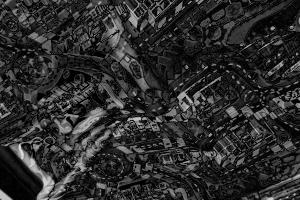
\includegraphics[width=\textwidth]{figures/rect_ru.jpg} 
    \caption{Original image (mean: 44.97).}
    \label{fig:rect_ru}
  \end{subfigure}
  \begin{subfigure}[b]{0.49\textwidth}
    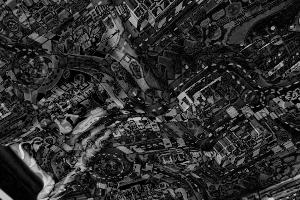
\includegraphics[width=\textwidth]{figures/rect_rw.jpg} 
    \caption{Rectified image (mean: 46.23).}
    \label{fig:rect_rw}
  \end{subfigure}
  \\
  \begin{subfigure}[b]{0.7\textwidth}
    
\includegraphics[width=\textwidth]{figures/rect_rdiff.jpg} 
    \caption{Difference of original and rectified image (mean: 6.71).}
    \label{fig:rect_rdiff}
  \end{subfigure}
  \caption{Rectification residual errors with $n_x = 300$ and $n_y = 200$.}
  \label{fig:rect}
\end{figure}


  % \chapter{Plane Dataset}
\section{Generation}

How plane dataset is created

\section{Shift Implementation}

How shift in x, y and z is implemented.



% \end{appendices}

%\nocite{*} %Show everything in bibliography.
% \bibliographystyle{siam}
% \bibliography{bibliography}

\end{document}
